\documentclass{ecnreport}

\stud{Control \& Robotics Master}
\topic{Manipulator Modeling \& Control}

\begin{document}

\inserttitle{Manipulator Modeling \& Control}

\section{Content of this lab}

The goal of this lab is to program in C++ the three fundamentals models for robot manipulators:
\begin{itemize}
	\item Direct Geometric Model: what is the pose of the end-effector for a given joint configuration?
	\item Inverse Geometric Model: what joint values correspond to a given end-effector pose?
	\item Kinematic Model: what is the velocity screw of the end-effector when the joints move?
\end{itemize}
These models will be applied on three different robots, and used to perform basic point-to-point control.\\

As it is not a lab on C++, most of the code is already written and you only have to fill the required functions:
\begin{itemize}
	\item \texttt{Robot::init\_wMe()} to initialize the fixed transform between the wrist and end-effector
	\item \texttt{Robot::fMw(q)} for the direct geometric model wrist-to-fixed frame
	\item \texttt{Robot::inverseGeometry(M)} for...well, the inverse geometry
	\item \texttt{Robot::fJw} for the kinematic model wrist-to-fixed frame
\end{itemize}

This project uses the ROS\footnote{Robot Operating System, http://www.ros.org} framework which imposes some particular steps to configure the environment. They are detailed in Appendix \ref{ros}.

The {\bf only} files to be modified are:
\begin{itemize}
	\item \texttt{control.cpp}: main file where the control is done depending on the current robot mode
	\item \texttt{robot\_turret.cpp}: model of the RRP turret robot
	\item \texttt{robot\_kr16.cpp}: model of the industrial Kuka KR16 robot
	\item \texttt{robot\_ur10.cpp}: model of the Universal Robot UR-10
\end{itemize}
We will use the ViSP\footnote{Visual Servoing Platform, http://visp.inria.fr} library to manipulate mathematical vectors and matrices, including frame transforms, rotations, etc. The main classes are detailed in Appendix \ref{visp}.\\

\section{The robots}

Three robots are proposed with increasing complexity. You should start with the Turret, then the Kuka KR16 then the UR-10.\\
For each of these robots, the table of Modified Denavit-Hartenberg parameters should be defined. As we saw during the lectures, once you have the table then the Direct Geometric and Direct Kinematic Models can be almost automatically derived. A tool is provided in this package to generate C++ code for the Geometric and Kinematic models, see Appendix \ref{dhcode} for details on this tool.

The robots are detailed in Appendix \ref{robots}. The fixed frame and the end-effector frames are imposed by the schematics. 
All intermediary frames have to be placed according to MDH convention, with a final fixed transform between the wrist and end-effector frames.

\subsection{Running the simulation}

Once everything is installed and compiled (see Appendix \ref{ros}), the base simulation can be run from a terminal (only 1 line depending on the robot you work on):
\cppstyle
\begin{lstlisting}
roslaunch ecn_manip turret.launch
roslaunch ecn_manip kr16.launch
roslaunch ecn_manip ur10.launch
\end{lstlisting}

\subsection{Direct Geometric Model}

\def\eMw{{}^e\M_w}

The first part is to build the direct geometric model, depending on the current value of $\q$. This is to be done in two functions:
\begin{itemize}
	\item \texttt{Robot::init\_wMe()} where you have to write the constant matrix $\eMw$ from the end-effector to the wrist frame
	\item \texttt{Robot::fMw(q)}  where you have to write and return the transform $\M$ between the fixed and wrist frame
\end{itemize}

\section{Building the models}




\appendix


\section{How to load the C++ project inside Qt Creator}\label{ros}

An actual ROS course will be held in the second semester, for now just configure as follows.\\
You should have a folder named \texttt{ros} in your home directory. Open a terminal inside and follow these steps:
\begin{enumerate}
	\item Clone this project inside  \texttt{ros/src}
	\begin{center}\cppstyle
		\begin{lstlisting}
		cd ~/ros
		mkdir src
		cd src
		git clone https://github.com/oKermorgant/ecn_manip.git
		\end{lstlisting}
	\end{center}
	\item Compile using catkin (you'll discover soon enough what it is) : \texttt{catkin build}
	\item Run Qt Creator from the top icon
	\item Load the \texttt{ros/src/ecn\_manip/CMakeLists.txt} file through \texttt{File...open project}
	\item QtCreator asks for a compilation folder: give \texttt{ros/build/ecn\_manip}
	\item The files should be displayed and ready to compile and run
	\item Compilation is done by clicking the bottom-left hammer
	\item Run your program with the green triangle. It can be stopped by clicking on the red square
	
\end{enumerate}

\section{Robots to be modeled}\label{robots}


\subsection{Turret RRP robot}

\begin{minipage}{.8\linewidth}
	This is a very simple robot to begin the modeling, as shown in the figure.\\
	The fixed frame $\Frame{0}$ and end-effector frame $\Frame{e}$ are imposed, as well as the joint direction.\\
	The constant values for this model are: $b = 0.5$ m and $d = 0.1$ m.	
\end{minipage}
\begin{minipage}{.2\linewidth}
	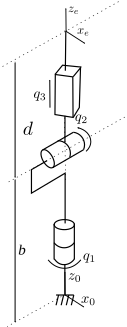
\includegraphics{fig/turret}\label{turret}
\end{minipage}

\subsection{Kuka KR16 anthropomorphic robot}

This robot is a classical 6R architecture with a spherical wrist, as shown in the next figure:

\begin{figure}[h!]\centering
	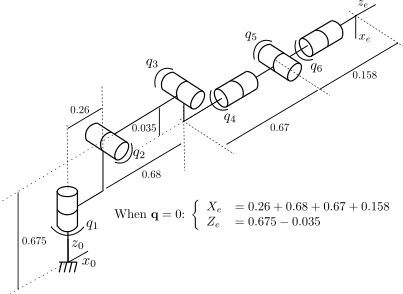
\includegraphics[width=.6\linewidth]{fig/kr16}
	\caption{Model of the Kuka KR16 with imposed fixed and end-effector frames}
\end{figure}

\newpage
\section{Using ViSP}\label{visp}


\newpage
\section{Code generation from Modified Denavit-Hartenberg parameters}\label{dhcode}

The core of robot modeling is to build the MDH table. From this, the DGM and KM can be derived automatically. The Inverse Geometry still has to be done by hand (even if some advanced tools allow code-generation for the IG resolution).

As it is quite tedious to have to recompute all matrices when a solution of MDH is investigated, a tool is provided to generate the C++ code. An example can be found in the file \texttt{dh\_example.yml}:
\cppstyle
\begin{lstlisting}
notation: [alpha, a, theta, r]
joint:
1: [0, 0, q1, 0]
2: [-pi/2, 0, 0, q2]
3: [pi/2, 0, q3, r3]
4: [-pi/2, a4, q4+pi/2, 0]
\end{lstlisting}
The command to be run is: \texttt{rosrun ecn\_manip dh\_code.py <name of the file>}.\\
In the case of the above MDH table, it leads to these outputs:

\begin{minipage}{.45\linewidth}
\cppstyle \raggedright
\begin{lstlisting}
// Generated pose code                                                                                                                                                                                                                  
const double c1 = cos(q[0]);                                                                                                                                                                                                            
const double c1p3 = cos(q[0]+q[2]);                                                                                                                                                                                                     
const double c4 = cos(q[3]);                                                                                                                                                                                                            
const double s1 = sin(q[0]);                                                                                                                                                                                                            
const double s1p3 = sin(q[0]+q[2]);                                                                                                                                                                                                     
const double s4 = sin(q[3]);                                                                                                                                                                                                            
M[0][0] = -s4*c1p3;                                                                                                                                                                                                                     
M[0][1] = -c4*c1p3;                                                                                                                                                                                                                     
M[0][2] = -s1p3;                                                                                                                                                                                                                        
M[0][3] = a4*c1p3 - q[1]*s1;                                                                                                                                                                                                            
M[1][0] = -s4*s1p3;
M[1][1] = -s1p3*c4;
M[1][2] = c1p3;
M[1][3] = a4*s1p3 + q[1]*c1;
M[2][0] = -c4;
M[2][1] = s4;
M[2][2] = 0;
M[2][3] = r3;
M[3][0] = 0;
M[3][1] = 0;
M[3][2] = 0;
M[3][3] = 1.;
// End of pose code
\end{lstlisting}
\end{minipage}
\begin{minipage}{.1\linewidth}
	\quad\quad
\end{minipage}
\begin{minipage}{.45\linewidth}
\cppstyle \raggedright
\begin{lstlisting}
// Generated Jacobian code
const double c1 = cos(q[0]);
const double c1p3 = cos(q[0]+q[2]);
const double s1 = sin(q[0]);
const double s1p3 = sin(q[0]+q[2]);
J[0][0] = -a4*s1p3 - q[1]*c1;
J[0][1] = -s1;
J[0][2] = -a4*s1p3;
//J[0][3] = 0;
J[1][0] = a4*c1p3 - q[1]*s1;
J[1][1] = c1;
J[1][2] = a4*c1p3;
//J[1][3] = 0;
//J[2][0] = 0;
//J[2][1] = 0;
//J[2][2] = 0;
//J[2][3] = 0;
//J[3][0] = 0;
//J[3][1] = 0;
//J[3][2] = 0;
J[3][3] = -s1p3;
//J[4][0] = 0;
//J[4][1] = 0;
//J[4][2] = 0;
J[4][3] = c1p3;
J[5][0] = 1.;
//J[5][1] = 0;
J[5][2] = 1.;
//J[5][3] = 0;
// End of Jacobian code
\end{lstlisting}	
\end{minipage}
This is exactly what you would get by doing the manual computation from the initial table, which I hope is quite appreciated.







\end{document}
